%
% Template de projeto de disserta��o
% Programa de P�s-Gradua��o em Engenharia da Computa��o (ppgec) 
% Escola Politecnica de Pernambuco
% Universidadede Pernambuco
% Recife Pernambuco Brasil
% 22 de Julho de 2013
% 
% Autor: Carlos Henrique Maciel Sobral Tim�teo
%

\documentclass[a4paper,12pt]{article}

\usepackage[latin1]{inputenc}

\usepackage{amsfonts}
\usepackage{amssymb}
\usepackage[portuguese,brazilian]{babel}
\usepackage{graphicx}
\usepackage{float}
\usepackage{units}
\usepackage{placeins}
\usepackage{subfig}
\usepackage{listings}
\usepackage{tabularx,colortbl}
\usepackage{color}
\definecolor{gray}{rgb}{0.6,0.6,0.6}

\usepackage[tmargin=1.5cm]{geometry}
\usepackage{fancyhdr}

\pagestyle{fancy}
\fancyhead{}
\fancyfoot{}

\fancyhead[L]{
  	\parbox{2cm}{\includegraphics[scale=0.4]{image/poli_logo_white.jpg}}
}

\fancyhead[R]{
		\parbox{1cm}{\includegraphics[scale=0.4]{image/upe_logo_white.jpg}} 
}

\fancyfoot[R]{
		\parbox{5.0cm}{\footnotesize {\color{gray}{PPGEC UPE/POLI - Page \thepage}}  }  
}

\renewcommand{\headrulewidth}{0.0pt}
\renewcommand{\footrulewidth}{0.0pt}
\setlength{\headheight}{80.0pt}
\fancyheadoffset[LO]{3.0cm}
\setlength{\textheight}{650.0pt}


\begin{document}
	\begin{titlepage}
	\begin{figure}[ht]
	  \mbox{\includegraphics[scale=0.4]{image/poli_logo.jpg}}\hfill
	  \mbox{\includegraphics[scale=0.4]{image/upe_logo.jpg}}
  \end{figure}
  \begin{center}
	  \textbf{Programa de P�s-Gradua��o em Engenharia da Computa��o}\\[1cm]
  	\includegraphics[scale=0.2]{image/ecomp_logo.jpg}\\[4cm]
	
	\textbf{Uma Abordagem para An�lise de Risco no Gerenciamento de Projetos de Software}\\[2cm]

	Mestrado Acad�mico\\[0.1cm]
	Engenharia da Computa��o\\[1cm]
	** \textbf{2� Estudo} **\\[2cm]

  \end{center}

  \begin{center}
    Carlos Henrique Maciel Sobral Tim�teo\footnote{Email: chmst@ecomp.poli.br}\\
    S�rgio Murilo Maciel Fernandes\footnote{Email: smurilo@ecomp.poli.br}\\
    M�user Jorge Silva Valen�a\footnote{Email: mjsv@ecomp.poli.br}\\[1cm]
  \end{center}
\end{titlepage}


	\section{Descri��o do Problema}

Risco � um conceito que muitos consideram dif�cil de ser compreendido: uma medida da probabilidade e da severidade de efeitos adversos \cite{Haimes2009}. Uma limita��o dessa defini��o � a dificuldade pr�tica em estimar a probabilidade e o impacto de diversos fatores de risco, especialmente em projetos de software. As probabilidades somente podem ser definidas com signific�ncia para atividades que s�o repetidas muitas vezes sob circunst�ncias controladas, no entanto, a natureza �nica de muitas atividades de projetos de software n�o permite a estimativa precisa de suas probabilidades. Uma abordagem cl�ssica na teoria da decis�o \cite{bannerman2008risk} define risco como uma varia��o numa distribui��o de probabilidade de resultados, n�o um resultado prov�vel.

Outra limita��o dessa defini��o � que ela abrange somente amea�as conhecidas ou previs�veis, oferecendo op��es limitadas para gerenciar amea�as n�o percebidas, como tamb�m, n�o reconhece amea�as imprevis�veis. Essa � uma consequ�ncia da defini��o de risco em termos de probabilidade e impacto; j� que, para avaliar a probabilidade e o impacto � necess�rio ser capaz de prever uma eventualidade \cite{bannerman2008risk}.

Al�m disso, existe outra quest�o: as melhores decis�es s�o baseadas na quantifica��o num�rica - determinada pelos padr�es do passado - ou na avalia��o subjetiva das incertezas? N�o � poss�vel quantificar o futuro com certeza, mas atrav�s da probabilidade, � poss�vel prev�-lo a partir do passado. Apesar de ser dif�cil encontrar um projeto de software padr�o, � poss�vel classificar atividades e definir padr�es que possibilitem a estimativa. Para Bannerman \cite{bannerman2008risk}, a solu��o comum para esse problema em projetos de software � observar o risco de um modo mais geral, em termos da incerteza, e avali�-lo qualitativamente. 

Haimes \cite{Haimes2009} considera duas premissas na pesquisa de an�lise de riscos, que tamb�m ser�o consideradas neste estudo. Uma, que o risco � comumente quantificado atrav�s da f�rmula matem�tica de expectativa. No entanto, mesmo que essa f�rmula permita uma medida valiosa do risco, ela falha em reconhecer e/ou acentuar consequ�ncias de eventos extremos. Tom Kendrick apresenta no seu livro \cite{KEND2003BOOK} um \textit{framework} para a identifica��o e gerenciamento de cat�strofes. A outra, por sua vez, afirma que uma das tarefas mais dif�cil em an�lise de sistemas � saber como model�-lo. Portanto, novas propostas para a an�lise quantitativa e modelagem de sistemas sob o ponto de vista de seus riscos contribuir�o para o avan�o cient�fico da �rea.

Os processos realizados na fase de execu��o de projetos de software s�o atividades de alto risco, ocasionando resultados com desempenho vari�vel. Uma pesquisa na ind�stria \cite{bannerman2008risk} sugere que somente cerca de um quarto dos projetos de software alcan�am sucesso - isto �, eles finalizam dentro do cronograma, no or�amento e como especificado - e bilh�es de d�lares s�o perdidos anualmente atrav�s de falhas de projeto ou projetos que n�o entregam os benef�cios prometidos. Evid�ncias sugerem que isso � um problema global \cite{KPMG2005}, impactando organiza��es do setor p�blico e privado.

Embora o gerenciamento de risco na gest�o de projetos de software seja um processo saud�vel, sua utiliza��o ainda est� aqu�m das expectativas. Algumas causas disso s�o o ac�mulo de responsabilidades dos gerentes de projetos, a baixa import�ncia atribu�da a essa �rea, a falta de conhecimento em gest�o de riscos, os custos envolvidos nas atividades de gest�o de risco, a falta de habilidade para lidar com as t�cnicas e ferramentas espec�ficas. Como consequ�ncia, o projeto est� sujeito � influ�ncia negativa de riscos sem haver um plano de conting�ncia, o que pode ocasionar o fracasso do projeto. De acordo com o \textit{benchmarking} realizado em 2009 pelo \textit{Project Management Institute} \cite{BENCHMARK2009}, em 20\% dos projetos seus gerentes n�o realizam todos os processos de planejamento; 46\% dos gerentes realizam atividades de gerenciamento em tempo parcial; apenas 35\% dos projetos o gerenciamento de riscos � realizado de acordo com uma metodologia formal, estruturada por pol�ticas, procedimentos e formul�rios.

\section{Objetivos}

\subsection{Quest�es da Pesquisa}

Como definir e modelar os riscos no gerenciamento de projetos de software, tamb�m considerando as cat�strofes? \\
Como analisar quantitativamente os risco no gerenciamento de projetos de software? \\
Quais os dados dispon�veis de registros de riscos de projetos de software para realizar os estudos? \\
Como desenvolver um modelo para previs�o de riscos em gerenciamento de projetos de software eficiente para o suporte a tomada de decis�o? \\

\subsection{Objetivo Geral}

O objetivo geral deste projeto de mestrado est� associado � pesquisa e desenvolvimento de uma nova abordagem para a an�lise de risco no gerenciamento de projetos de software, baseado em t�cnicas de computa��o inteligente e em formalismos matem�ticos para a modelagem de sistemas din�micos. 

\subsection{Objetivos Espec�ficos}
\begin{itemize}
  \item Desenvolver uma t�cnica baseada em Redes de Petri para a previs�o da probabilidade de riscos em gerenciamento de projetos de software
  \item Desenvolver uma t�cnica para a previs�o do impacto dos riscos baseada em computa��o inteligente para o gerenciamento de riscos de projetos de software
  \item Desenvolver um m�todo para o suporte a tomada de decis�o para a defini��o de estrat�gias de mitiga��o de riscos e seu gerenciamento em projetos de software
\end{itemize}

\section{Motiva��o}

Existe uma dificuldade na interpreta��o do conceito de risco. Principalmente quanto a aplica��o desse conhecimento no desenvolvimento e utiliza��o de t�cnicas eficientes para a an�lise de risco no gerenciamento de projetos de software. A gest�o de riscos e incertezas em projetos de software, � fundamental para a disciplina de gerenciamento de projetos. Entretanto, em momentos econ�micos de crise torna-se muito mais dif�cil realizar o gerenciamento de riscos, devido aos custos incorridos.

Em 2009, o CHAOS Report \cite{CHAOS2009} mostrou que 32\% dos projetos alcan�aram sucesso - foram entregues no prazo, no or�amento e com os requisitos prometidos -, 44\% dos projetos foram desafiados; n�o menos importante, 24\% dos projetos falharam e foram cancelados. Isso ocorre devido aos riscos envolvidos nas atividades e a um gerenciamento de risco de software ausente ou deficiente \cite{ISLAM2009}. 

Como prever poss�veis eventos a curto, m�dio e longo prazos? Ao analisar os riscos e incertezas, os gerentes de projeto muitas vezes confiam na intui��o, em vez de l�gica e an�lise detalhada. No entanto, o pensamento intuitivo � frequentemente alvo de ilus�es, que causam erros mentais previs�veis e decis�es eventualmente pobres. O m�todo para conciliar o efeito dessas ilus�es psicol�gicas � uma avalia��o sistem�tica dos riscos e esfor�os na mitiga��o dos mesmos atrav�s de m�todos anal�ticos. � dif�cil gerenciar algo que n�o pode ser medido: gerentes de projeto deveriam quantificar a probabilidade de risco, os resultados, e seu efeito cumulativo em um projeto. Al�m disso, � importante avaliar as v�rias op��es de mitiga��o: o custo de cada op��o e o tempo necess�rio para a realiza��o da mitiga��o \cite{VIRINE2009}.

J� que � uma �rea de pesquisa que vem crescendo, novas e melhores metodologias para identificar, medir e controlar itens de risco de software precisam ser desenvolvidas. Keshlaf e Riddle \cite{KESHLAFRIDDLE2010} concluem que mesmo que existam muitas abordagens ainda h� uma grande lacuna com rela��o ao que � praticado pelas ind�strias de software. Al�m disso, vale a pena perceber que n�o existe uma solu��o �nica para o conduzir o gerenciamento de riscos adequadamente \cite{VIRINE2009}. 

Alguns benef�cios da boa gest�o de riscos de projetos de software s�o: a redu��o de custos incorridos com mudan�as no software; o desenvolvimento de um plano de respostas a eventos inesperados, ou seja, um plano de conting�ncia de riscos; a previs�o da probabilidade da ocorr�ncia de eventos indesejados; o seguimento das linhas de base de custo, cronograma e qualidade. Tais fatores podem determinar o sucesso dos projetos \cite{HIGUERAHAIMES1996} \cite{PMBOK2008}.


\section{Estado da Arte}

A Ger�ncia de Riscos de Projetos foi formalmente apresentada � comunidade de Engenharia de Software atrav�s da proposta do modelo Espiral de Barry Boehm \cite{BOEHM1991}. Seguindo-se a esse evento muitas abordagens e modelos foram apresentados, destacando-se o programa do SEI (\textit{Software Engineering Institute}) \cite{HIGUERAHAIMES1996} e, atualmente, os mais conhecidos modelo CMMI (\textit{Capability Maturity Model Integration}) \cite{SEI2007} e o Guia PMBOK (\textit{Project Management Book of Knowledge}) \cite{PMBOK2008}.

O Gerenciamento de riscos de projetos � um dos principais t�picos de interesse dos pesquisadores e trabalhadores da �rea de gerenciamento de projetos. Tanto que um \textit{survey} realizado por Williams em 1995 \cite{WILLIAMS95} inclui 241 refer�ncias.

\subsection{Gerenciamento de Riscos de Projetos}

O Gerenciamento de Risco envolve processos de planejamento, identifica��o, avalia��o e prioriza��o dos mesmos. De acordo com o PMBOK \cite{PMBOK2008}, riscos podem ser definidos como um evento incerto ou condi��o que, se ocorrer, tem um efeito em pelo menos um dos objetivos do projeto. Ele pode ser considerado tanto como amea�a (impacto negativo) ou oportunidade (impacto positivo). Numa defini��o melhor, gerenciamento de riscos pode ser definido como o processo de analisar a exposi��o ao risco e determinar como melhor lidar com essa exposi��o. Um objetivo dessa �rea n�o � somente a identifica��o, mas tamb�m desenvolver uma abordagem robusta para gerenciar proativamente o impacto no projeto \cite{OSUNDAHUNSI2012}.

Para o PMBOK \cite{PMBOK2008}, os processos de gerenciamento de risco do projeto s�o direcionados para aumentar a probabilidade e o impacto de eventos que s�o esperados para afetar positivamente o projeto, bem como para diminuir o probabilidade e o impacto dos eventos que s�o esperados para negativamente afetar o projeto ou a realiza��o de seus objetivos. 

O Software Engineering Institute(SEI) desenvolveu uma metodologia de gerenciamento de risco chamada \textit{Software Risk Evaluation}(SRE) que � especificamente voltada para projetos na ind�stria de software. O paradigma SRE � composto por seis elementos: cinco m�dulos (identificar, analisar, planejar, acompanhar, controlar) e um elemento central (comunica��o), que � a chave para a efetiva gest�o de riscos \cite{HIGUERAHAIMES1996} \cite{williams1999software}.

Boehm \cite{BOEHM1991}, Chapman \cite{chapman1996project}, Fairley \cite{fairley1994risk}, Bandyopadhyay et al. \cite{bandyopadhyay1999framework} apresentaram m�todos e modelos diferentes de gerenciamento de riscos de projetos de software. No entanto, h� elementos em comum em todas as abordagens anteriores: a identifica��o, a avalia��o da probabilidade e impacto, e o planejamento a respostas para manusear esses riscos se eles ocorrerem \cite{holzmann2011developing}.

\subsubsection{An�lise Qualitativa de Riscos em Projetos}

O processo de an�lise qualitativa avalia as caracter�sticas dos riscos de projetos identificados individualmente e prioriza-os baseado nas requisi��es estabelecidas para o projeto. Em outras palavras, a an�lise qualitativa avalia a probabilidade de cada evento ocorrer e o efeito individual de cada um deles nos objetivos do projeto. Como tal processo n�o aborda diretamente o risco global para os objetivos do projeto, que resultam do efeito combinado dos eventos individuais e suas intera��es entre si, ent�o isso pode ser obtido atrav�s do uso de t�cnicas de an�lise quantitativa \cite{PRACTICESTANDARD2009}.

\subsubsection{An�lise Quantitativa de Riscos em Projetos}

A an�lise quantitativa de riscos envolve o processo de mapear eventos de riscos relacionados a atividades e executar a simula��o de Monte Carlo considerando a probabilidade de ocorr�ncia.

O objetivo da an�lise quantitativa de riscos � criar um "perfil do risco" do projeto. Para tanto, s�o necess�rias as seguintes informa��es: a chance de o projeto ser finalizado dentro de um certo per�odo de tempo ou or�amento; a taxa de sucesso de projetos; as estimativas pior, m�dia e melhor de dura��o e outros par�metros do projeto \cite{PMBOK2008}.

As ferramentas utilizadas na an�lise quantitativa s�o:
\begin{enumerate}
  \item An�lise de Sensibilidade: determina qual incerteza tem o maior potencial de impacto.
  \item Simula��o de Monte Carlo: m�todo matem�tico utilizado para aproximar a fun��o de distribui��o de probabilidade de resultados potenciais (dura��o do projeto, custo, taxas de sucesso, e outros par�metros baseado em entradas probabil�sticas). Nesse procedimento amostras aleat�rias s�o criadas com base na amostra apresentada, de modo que a fun��o de distribui��o de probabilidade alcance o n�vel de confian�a desejado, comummente 95\% ou 99\%.
  \item An�lise de �rvore de Falha: tipo de an�lise que determina qual decis�o � a melhor. Por exemplo, para o gerenciamento do custo do projeto, a �rvore de decis�o suporta o c�lculo do Valor Monet�rio Agregado (\textit{Estimated Monetary Value}) que determina qual decis�o � menos onerosa.
\end{enumerate}
 
Alguns trabalhos prop�em novas ferramentas de an�lise quantitativa de riscos. Entre eles, Virine \cite{VIRINE2009} apresenta a metodologia da Cadeia de Eventos. Nesse trabalho, as atividades de um projeto n�o s�o um procedimento uniforme e cont�nuo, essas tarefas s�o afetadas por eventos externos, que transformam as atividades de um evento para outro. O momento em que os eventos externos ocorrem s�o probabil�sticos e podem ser definidos utilizando uma distribui��o estat�stica. Al�m disso, eventos podem causar outros eventos, criando, portanto, a Cadeia de Eventos. A an�lise dessas combina��es � realizada atr�ves da simula��o de Monte Carlo.




\subsection{T�cnicas Convencionais de An�lise de Risco}

\subsubsection{Simula��o de Monte Carlo}

A inven��o desse m�todo, especialmente o uso de computadores para fazer os c�lculos, foi creditado a Stanislaw Ulam, um matem�tico trabalhando no Projeto Americano de Manhattan durante a Segunda Guerra Mundial. O seu trabalho com Jon von Neuman e Nicholas Metropolis transformou a amostragem estat�stica de uma curiosidade matem�tica para uma metodologia formal aplic�vel a uma grande variedade de problemas \cite{kwak2007exploring}. 

Simula��o de Monte Carlo � uma abordagem detalhada de simula��o atrav�s de computa��o intensiva para determinar a probabilidade de resultados poss�veis de um objetivo do projeto; por exemplo, a data de conclus�o ou o custo total. As entradas para o procedimento s�o obtidas aleatoriamente a partir de intervalos espec�ficos com fun��es de distribui��o de probabilidade para as dura��es das atividades do cronograma ou itens da linha de custo. Esses valores de entrada diferentes s�o usados para construir um histograma de poss�veis resultados do projeto e sua probabilidade relativa, como tamb�m, a probabilidade cumulativa para calcular as reservas de conting�ncia desejadas de tempo ou custo. Resultados adicionais incluem a import�ncia relativa de cada entrada na determina��o do custo geral do projeto e cronograma. Um exemplo de resultados de estimativa de riscos de cronograma e custo s�o apresentados na Figura \ref{fig:montecarlo} \cite{PRACTICESTANDARD2009}.

Esse m�todo tem sido utilizado em projetos de constru��o para entender melhor certos riscos do projeto. Por exemplo, o ru�do e seus efeitos negativos sobre a comunidade no entorno de uma obra � um risco em muitos projetos de constru��o urbana. Nesse caso, o modelo de simula��o de Monte Carlo permite aos construtores prever e mitigar a ocorr�ncia e o impacto do ru�do da constru��o \cite{kwak2007exploring} \cite{PRACTICESTANDARD2009}.

Na Figura \ref{fig:montecarlo}, observa-se a previs�o de finaliza��o para um cronograma de um projeto. No eixo horizontal, encontram-se as poss�veis datas de finaliza��o do cronograma, a frequ�ncia de ocorr�ncia dessas datas na amostragem s�o representada pelas barras verticais, a frequ�ncia cumulativa � representada pela curva escura e pelos respectivos valores na borda direita do gr�fico. A partir da frequ�ncia relativa, � poss�vel prever a probabilidade do projeto finalizar at� determinada data, por exemplo, esse projeto tem 90\% de chance de finalizar at� 08 de Maio de 2009.

\begin{figure}[H]
	\centering
	\includegraphics[width=.6\textwidth]{image/montecarlo.png}
	\caption{Exemplo de Resultado da Simula��o Monte Carlo}
	\label{fig:montecarlo}
\end{figure}

\subsubsection{An�lise de �rvore de Falha ou An�lise de Modos de Falha e Efeitos}

An�lise de �rvore de Falha, do ingl�s \textit{Fault Tree Analysis} (FTA), � um m�todo importante para analisar e estimar a confiabilidade e disponibilidade de um sistema. No processo de concep��o do sistema, depois de analisar v�rios fatores de fracasso (como \textit{hardware}, \textit{software}, ambiente, fatores individuais), podemos construir o diagrama l�gico (isto �, a �rvore de falha), sequencialmente, identificando todas as causas para prever a probabilidade de falha do sistema e tomar medidas corretivas para melhorar a confiabilidade e seguran�a \cite{yu2009application}.

No processo de constru��o da �rvore de falha, um efeito indesejado � tomado como alvo na an�lise l�gica, chamado de "evento de topo"; e, em seguida, todas as poss�veis causas diretas desse efeito indesejado s�o descobertas, rotulados de "eventos do meio"; sequencialmente, todas as poss�veis causas diretas desses "eventos do meio", chamados de "eventos de fundo". O diagrama l�gico em �rvore, que normalmente � escrito usando s�mbolos de portas l�gicas e eventos de topo, do meio e de fundo, � chamado de �rvore de Falha \cite{yu2009application}.

De modo geral, a constru��o da �rvore de Falha � dividida em quatro passos: 
\begin{enumerate}
  \item Selecionar e obter o evento de topo. O evento de topo � o evento indesejado, ou o evento de falha da an�lise l�gica da linha destacada. 
  \item Analisar o evento de topo. Descobrir todas as causas diretas, necess�rias e suficientes do evento de topo. Tome o evento de topo como o evento de sa�da e todos os motivos diretos como eventos de entrada, e interligue esses eventos usando portas l�gicas apropriadas de acordo com as suas rela��es l�gica atuais. 
  \item Analisar todos os eventos de entrada diretamente ligado ao evento de topo. Tome-o como evento de sa�da do pr�ximo n�vel se o evento pode ser decomposto adiante, como realizado no passo 2. 
  \item Repetir os passos acima, decomponha-os passo a passo at� que todos os eventos de entrada n�o possam ser desmontados ou n�o precisam ser quebrados, isso � uma �rvore de falha completamente invertida, como mostrado na Figura \ref{fig:faulttree} \cite{yu2009application}:
\end{enumerate}

Na Figura \ref{fig:faulttree}, observa-se uma �rvore de falha com um "evento de topo", tr�s "eventos do meio" (A1,A2 e A3), "seis eventos" de fundo (B1 a B6), uma porta l�gica "E" (T1) e tr�s portas l�gicas "OU" (T2, T3 e T4). Essa �rvore de falha representa o seguinte conhecimento: O evento de topo ocorre, se os eventos A1, A2 e A3 ocorrerem. O evento A1 ocorre, se os eventos B1 ou B2 ocorrerem. O evento A2 ocorre, se os eventos B3 ou B4 ocorrerem. O evento A3 ocorre, se os eventos B5 ou B6 ocorrerem.

\begin{figure}[H]
	\centering
	\includegraphics[width=.3\textwidth]{image/faulttree.png}
	\caption{Exemplo de �rvore de Falha}
	\label{fig:faulttree}
\end{figure}


\subsection{T�cnicas Estat�sticas e de Computa��o Inteligente para An�lise de Risco}

\subsubsection{Rede Bayesiana}

Rede Bayesiana pertence � fam�lia de modelos gr�ficos probabil�sticos. Uma rede bayesiana $B$ � um grafo ac�clico direto (GAD) que representa uma distribui��o de probabilidade combinada sobre um conjunto de vari�veis aleat�rias $V$, no qual os n�s representam vari�veis e as arestas expressam as depend�ncias entre vari�veis \cite{jensen1996introduction}. Logo, a rede pode ser definida por um par $B=<G,\Theta>$ , em que $G$ � o GAD cujos n�s $X_1,X_2,...,X_n$ representam vari�veis aleat�rias, e cujas arestas representam as depend�ncias diretas entre vari�veis. Baseado em premissas independentes, cada n� $X_i$ no grafo $G$ � dependente de seus pais em $G$. Logo, o grafo $G$ leva em considera��o a Suposi��o Markoviana \cite{li2012integrated}. A Suposi��o Markoviana para uma rede bayesiana estabelece que qualquer n� nessa rede � condicionalmente independente de seus n�o descendentes, dado que existe um parentesco. $\Theta$ representa o conjunto de par�metros da rede bayesiana, que cont�m par�metros $\theta_{X_i|\pi} = P_B(X_i|\pi_i)$ para cada valor $x_i$ do n� $X_i$ condicionando a $\pi_i$, onde $\pi_i = parent(X_i)$ \cite{neal1993probabilistic}. 

Essa t�cnica tem sido usada como uma ferramenta importante para explorar diferentes informa��es, incluindo informa��es determin�sticas ou probabil�sticas de rela��es complexas entre vari�veis. Elas constituem um \textit{framework} de pesquisa conveniente que � f�cil de usar pelos especialistas, principalmente na �rea de confiabilidade. Em particular, interesses de pesquisa significantes existem no uso de modelos de redes bayesianas para a an�lise de confiabilidade de sistemas e risco em engenharia de software, como tamb�m previs�o de qualidade \cite{li2012integrated} \cite{fenton2007predicting}.

Atrav�s do aprendizado da rede bayesiana, todas as probabilidades condicionais entre cada dois riscos adjacentes podem ser calculadas. Uma rede bayesiana, pode n�o somente capturar o relacionamento entre convic��es incertas em proposi��es, mas tamb�m pode explicar o valor de verdade de uma ou mais proposi��es. Algoritmos de infer�ncia da rede bayesiana podem ser usados para encontrar causalidades ou cren�as atualizadas para cada uma das vari�veis, e rela��es atualizadas entre vari�veis \cite{jensen2007bayesian}. Uma rede bayesiana codifica a distribui��o de probabilidade de um conjunto de vari�veis aleat�rias atrav�s da especifica��o de um conjunto de suposi��es de independ�ncia ou deped�ncia condicional junto com um conjunto de relacionamentos entre essas vari�veis e suas probabilidades combinadas relacionadas. Ao inv�s de resultados determin�sticos tipicamente gerados pelo aprendizado, redes bayesianas podem produzir um conjunto de resultados probabil�sticos em cada processo. Eles s�o mais adequados para a identifica��o de riscos em diferentes fases do processo de software em situa��es reais \cite{li2012integrated}.

A Figura \ref{fig:bayesian} ilustra um exemplo de uma rede bayesiana simples para um projeto com tr�s tipos de fatores de risco e dois subprocessos. Identificados pelo �ndice $R_{ij}$, onde $i$ representa os tipos de fatores de risco e $j$ representa o n�mero de subprocessos. Ele inclui tr�s n�s pais e tr�s n�s filhos.

%TROCAR o EXEMPLO

\begin{figure}[H]
	\centering
	\includegraphics[width=.6\textwidth]{image/bayesian.png}
	\caption{Exemplo simples de Rede Bayesiana}
	\label{fig:bayesian}
\end{figure}

\subsubsection{Redes de Petri Estoc�sticas}

A Rede de Petri � um formalismo matem�tico que permite representar sistemas din�micos em que h� rela��es de causa e efeito complexas, concorr�ncia e sincroniza��o. Elas foram criadas em 1962 por Carl Adam Petri \cite{PETRI1962}. A rede de Petri � um grafo direcionado em que h� dois tipos de n�s: lugares, representados por c�rculos, e transi��es, representadas por barras ou ret�ngulos. Os lugares podem conter tokens, que s�o representados por c�rculos pretos dentro do lugar. 

Em \cite{JIANGCHEN2004}, uma t�cnica baseada em redes de petri foi utilizada para a an�lise qualitativa e quantitativa de riscos em desenvolvimento de software. O artigo apresenta um \textit{framework} de coordena��o de m�tricas de software e modelo de processos de software para gerenciar os riscos de projetos. Al�m disso, \cite{CARDOSO2012} utilizou redes de Petri para identificar, controlar, e gerenciar riscos de desenvolvimento de programas.

A Figura \ref{fig:redespetri} apresenta um exemplo simples de rede de Petri, em que � modelado o ciclo dia e noite. Quando um \textit{token} � colocado no lugar Dia, significa que o sistema est� no estado Dia. Isto habilita a transi��o Anoitecer a ocorrer. Quando esta transi��o dispara, o \textit{token} � removido do lugar Dia e um \textit{token} � colocado no lugar Noite, indicando que o sistema est� neste estado. Isto, por sua vez, desabilita a transi��o Anoitecer e habilita a transi��o Amanhecer. De forma an�loga, o disparo da transi��o Amanhecer faz com que o \textit{token} seja removido do lugar Noite e um \textit{token} seja colocado no lugar Dia \cite{HirelTT00} \cite{MURILO2007}.

\begin{figure}[H]
	\centering
	\includegraphics[width=.6\textwidth]{image/redepetri.png}
	\caption{Exemplo de Rede de Petri}
	\label{fig:redespetri}
\end{figure}

As Redes de Petri Estoc�sticas Generalizadas (\textit{Generalized Stochastic Petri Nets}) \cite{MBEA1995}, permitem a utiliza��o de transi��es temporizadas estoc�sticas em conjunto com transi��es n�o-temporizadas (chamadas imediatas). Esta caracter�stica facilita a modelagem de transi��es l�gicas, que n�o est�o associadas a tempo. Transi��es temporizadas apenas s�o habilitadas quando n�o h� mais nenhuma transi��o imediata habilitada. Marca��es em que transi��es imediatas est�o habilitadas s�o chamadas de n�o-tang�veis (\textit{vanishing}). Marca��es em que transi��es temporizadas est�o habilitadas s�o chamadas de tang�veis (\textit{tangible}).

\subsubsection{Redes Neurais Artificiais}

As Redes Neurais Artificiais (RNA) s�o modelos que procuram simular o comportamento e funcionamento do c�rebro humano. Assim como existem os neur�nios biol�gicos, componentes essenciais para o processamento das informa��es do c�rebro, a RNA � formada por unidades que objetivam realizar as mesmas fun��es do neur�nio biol�gico. Esses componentes s�o denominados neur�nios artificiais e foram propostos em 1943 por Mc-Culloch e Pitts \cite{MCCULLOCKPITTS1943}.

\subsubsection{\textit{MultiLayer Perceptron}}
A rede \textit{MultiLayer Perceptron} (MLP) funciona como um \textit{perceptron} de muitas camadas, ou seja, ela possui pelo menos uma camada de neur�nios intermedi�ria ou escondida. A vantagem de ter camadas intermedi�rias � que a rede neural passa a resolver problemas que n�o s�o linearmente separ�veis, possibilitando, assim, a aproxima��o de qualquer fun��o cont�nua, com apenas uma camada, e qualquer fun��o matem�tica, quando houver mais de uma camada \cite{HAYKIN2007}. A Figura \ref{fig:mlp} ilustra a forma gr�fica da MLP, apresentando as entradas, sa�das e as camadas de entrada, intermedi�ria e de sa�da. 

\begin{figure}[H]
	\centering
	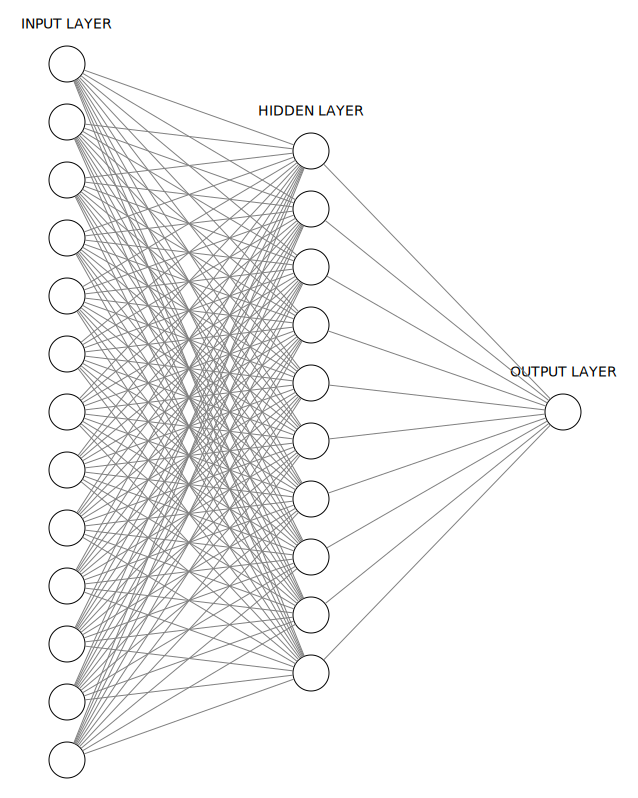
\includegraphics[width=.6\textwidth]{image/mlp.png}
	\caption{Representa��o gr�fica da MLP com tr�s camadas}
	\label{fig:mlp}
\end{figure}

O funcionamento da MLP � dividido em duas fases: \textit{forward} e \textit{backward}. Na fase \textit{forward}, um neur�nio de uma camada est� ligado a todos os neur�nios da camada seguinte. Os sinais da entrada s�o propagados de camada de entrada para a camada escondida e da camada escondida para a camada de sa�da; cada neur�nio processa as entradas e apresenta uma sa�da. Nessa fase � poss�vel calcular o erro entre a sa�da desejada para a rede e a sa�da apresentada pela MLP. Na fase \textit{backward} o erro � retropropagado e os pesos s�o ajustados, utilizando o algoritmo de ajustes de pesos, inicialmente aleat�rios, chamado \textit{Backpropagation} \cite{valenca2005aplicando}.

Em \cite{HUHUANG2007}, algumas t�cnicas inteligentes s�o utilizadas para a an�lise do risco projetos de software. O artigo conclui que uma t�cnica h�brida de redes neurais e algoritmos gen�ticos obteve uma precis�o de 85\% para prever se o projeto obter� sucesso, ser� desafiado ou falhar� totalmente.

\subsubsection{M�quina de Vetor de Suporte}

A M�quina de Vetor de Suporte, do ingl�s \textit{Support Vector Machine} (SVM), � uma t�cnica de aprendizado de m�quina aplic�vel a problemas de reconhecimento de padr�es nos quais se busca atingir alto potencial de generaliza��o \cite{HAYKIN2007} \cite{valenca2005aplicando}. O objetivo da SVM � encontrar um hiperplano particular, denominado de hiperplano �timo, que maximize a margem de separa��o, conforme pode ser visualizado na Figura \ref{fig:svm}.

Na Figura \ref{fig:svm}, observamos dois vetores de suporte capazes de separar linearmente as sa�das no hiperplano em duas classes. A vari�vel $r$ � a dist�ncia alg�brica desejada dos vetores de suporte para o hiperplano �timo de separa��o das classes. Quanto maior essa dist�ncia, maior a capacidade de generaliza��o da m�quina de vetor de suporte.

\begin{figure}[H]
	\centering
	\includegraphics[width=.6\textwidth]{image/svm.png}
	\caption{Vetores de Suporte e Hiperplano de Separa��o �timo}
	\label{fig:svm}
\end{figure}

\subsubsection{L�gica Fuzzy}

A aplica��o da Teoria de Conjuntos Fuzzy (TCF) para a an�lise de riscos parece apropriada, devido ao fato dessas an�lises serem altamente subjetivas e relacionadas a informa��es inexatas e vagas. Desde que TCF foi introduzida por Zadeh para lidar com problemas no qual imprecis�o era presente, valores lingu�sticos t�m sido amplamente usados para o racioc�nio aproximado. Numerosos estudos de TCF na avalia��o de risco tem surgido em diferentes �reas, e s�o sumarizados em \cite{ngai2005fuzzy}. TCF tem sido efetivo numa variedade de �reas porque ele pode lidar com informa��es inexatas, por�m �teis.

\subsubsection{\textit{Fuzzy Weight Average}}

Uma opera��o comumente usada em an�lise de risco e decis�o � a opera��o de m�dia ponderada, que tem a seguinte forma
 \cite{ngai2005fuzzy}:

\begin{equation}
	\bar{W} = \frac{\sum_{i=1}^{n}W_i \times R_i}{\sum_{i=1}^{n}W_i}
	\label{eq:fwa}
\end{equation}

onde $\bar{W}$ � a m�dia ponderada dos valores, $R_i$ � o valor de acordo com o crit�rio $i$, e $W_i$ � o peso atribu�do ao crit�rio $i$. Quando os termos $R_i$ e $W_i$ s�o representados por conjuntos fuzzy ou n�meros fuzzy, a opera��o acima � referenciada como uma M�dia Ponderada Fuzzy (MPF).

Schmucker \cite{schmucker1984fuzzy} usou a MPF para propor um m�todo n�merico aproximado conhecido como o "Analisador de Riscos Fuzzy". Al�m disso, muitas aplica��es seguem o procedimento de Schmucker, e isso � amplamente aplicado em an�lise de risco, particularmente com rela��o a projetos de constru��o \cite{ngai2005fuzzy}.

%introduzir melhor logica fuzzy a partir do Livro de Engelbrecht

\subsubsection{Conceitos de Confiabilidade}

% reescrever essa se��o, associando os conceitos de confiabilidade com o gr�fico de risco apresentado por Boehm

Se $X$ � uma vari�vel aleat�ria que indica o tempo de vida ou tempo at� a falha de um componente ou sistema e $X$ tem fun��o de distribui��o de probabilidade \cite{geist1990reliability}.

\begin{equation}
	F_X(t) = P(X \leq t)
	\label{eq:sobrevivencia}
\end{equation}

em seguida, a confiabilidade do componente ou sistema $R_X(t)$ representa a probabilidade de que o sistema sobreviva at� ao tempo $t$, isto �,

\begin{equation}
	R_X(t) = P(X < t) = 1 - F_X(t)
	\label{eq:confiabilidade}
\end{equation}

Se $R_X(t)$ � diferenci�vel, ent�o a taxa de perigo ou taxa de falha do componente ou sistema � dado por

\begin{equation}
	h(t) = -R_{X}^{'}(t) / R_X(t) = \frac{\partial F_X / \partial t}{1 - F_X(t)}
	\label{eq:perigo}
\end{equation}

a qual podemos interpretar vagamente como a taxa de falha condicional no pr�ximo instante dada a sobreviv�ncia at� t. Neste caso

\begin{equation}
	F_X(t) = 1 - e^{-\int_{0}^{t} h(x) dx}
	\label{eq:fx}
\end{equation}

e, portanto, uma taxa de falha constante implica uma distribui��o de tempo de vida exponencial.

Demandas para maior precis�o na estimativa de confiabilidade rapidamente for�ou o desenvolvimento de modelos de sistema mais elaborados sem os pressupostos de independ�ncia. A segunda gera��o de ferramentas de estimativa, surgiu com base em m�todos Markovianos, permitindo assim uma importante depend�ncia de primeira ordem.

Um modelo de Markov de estado discreto e tempo cont�nuo � um conjunto de estados, juntamente com as taxas de transi��o n�o negativas entre esses estados. Deixe $a_ij$, indicar a taxa de transi��o do estado $i$ para o estado $j$. O modelo de Markoviano representa ent�o um sistema em evolu��o o tempo que muda de estado de acordo com as seguintes regras \cite{geist1990reliability}:

\begin{enumerate}
   \item O tempo de espera em cada estado $i$ � exponencialmente distribu�do com m�dia $1 / \sum_{j \ne i}a_ij$
   \item Na sa�da do estado $i$, o estado $j$ � escolhido com probabilidade $a_ij / \sum_{j \ne i}a_ij$
\end{enumerate}

Esses modelos Markovianos s�o equivalentes a sistemas lineares de equa��es diferenciais ordin�rias especiais. Se $P_i(t)$ determina a probabilidade do sistema estar no estado $i$ no tempo $t$, $P(t) = (P_1(t),...,P_n(t)$, e $A$ � uma matriz $n \times n$ cujas entradas fora da diagonal s�o taxas de transi��o $a_ij$ e entradas diagonais $a_ii = - \sum_{j \ne i}a_ij$, ent�o o modelo markoviano � equivalente ao sistema linear homog�neo

\begin{equation}
	P^{'}(t) = P(t) A
	\label{eq:sistemalinearhomogeneo}
\end{equation}

Entre as ferramentas que utilizam um framework markoviano para constru��o e an�lise de modelos tolerante a falhas ou erros h� a rede de Petri \cite{geist1990reliability}. 

Por fim, Bonini e Caivano \cite{bonini2013} utilizaram os conceitos de sobreviv�ncia para desenvolver uma t�cnica de an�lise de risco de cr�dito. Essa abordagem mostrou-se bastante promissora no contexto de previs�o da quita��o de empr�stimos.


%A t�cnica de an�lise de sobreviv�ncia � usada numa variedade de contextos compartilhando uma caracter�stica comum: os interesses focam em descrever se, ou quando os eventos ocorrer�o \cite{stepanova2002survival}. Relacionando os conceitos apresentados em Bonini e Cavano \cite{keylist} sobre risco de cr�dito com risco de projetos, temos que a ocorr�ncia de um evento representa que o projeto est� mudando de um estado, cujos eventos de riscos n�o ocorreram, para um estado em que pelo menos um risco ocorreu e amea�a o sucesso do projeto. Na introdu��o de uma abordagem para sobreviv�ncia para riscos as seguintes premissas devem ser consideradas.

%\begin{itemize}
%   \item Uma gera��o de projetos � formada por projetos em incumprimento � data da observa��o.
%   \item O fracasso de um projeto ocorre quando um risco n�o pode ser mitigado.
%   \item O fracasso de um projeto � um evento incerto: a empresa n�o sabe se ou quando isso vai ocorrer.
%   \item O tempo de sobreviv�ncia do projeto � a diferen�a entre dois tempos: o tempo quando um evento de risco no projeto ocorre e o momento em que esse risco n�o pode ser mitigado.
%\end{itemize}

\section{Metodologia}


Esse projeto de pesquisa � realizado baseado nas seguintes atividades:

\begin{enumerate}
\item Pesquisa Bibliogr�fica das �reas de Conhecimento:
	\begin{itemize}
	\item Gerenciamento de Projetos
	\item Gerenciamento de Risco de Projetos
	\item An�lise de Risco de Projetos de Software
	\item Probabilidade e Estat�stica
	\item Confiabilidade de Sistemas
	\item M�todos Estat�sticos para An�lise de Risco
	\item M�todos Formais para An�lise de Risco
	\item Redes Neurais Artificiais
	\item Intelig�ncia de Enxames
	\end{itemize}
\item Levantamento de Bases de Dados com informa��es de Riscos de Gerenciamento de Projetos de Software
\item Levantamento de Ferramentas necess�rias para o Tratamento dos Dados contidos nas Bases
\item Defini��o de M�tricas Quantitativas e os Par�metros para An�lise de Risco de Projetos de Software
\item Avalia��o dos Resultados das M�tricas
\item Defini��o do Grau de Exposi��o ao Risco de um Projeto
\item Suporte a Tomada de Decis�es Estrat�gicas de Mitiga��o de Riscos
\end{enumerate}


\subsection{Base de Dados}

\subsubsection{Base de Dados PERIL}

Um melhor gerenciamento de riscos come�a com a identifica��o de problemas potenciais. A ado��o das ferramentas dispon�veis como: revis�o das li��es aprendidas, \textit{brainstorming}, entrevistas, opini�o especializada; s�o alternativas relativamente eficientes, por�m muitas vezes apresentam alto custo. Uma proposta acess�vel, de baixo custo e extens�vel � utilizar a base de dados do PERIL \cite{KEND2003BOOK}.

Durante alguns anos, em \textit{Workshops} de Gerenciamento de Riscos, foram realizadas entrevistas com centenas de l�deres de projetos para conhecer problemas de projetos t�picos j� enfrentados, definindo o que havia ocorrido e o impacto disso no projeto. Esses dados foram agrupados no banco de dados \textit{Project Experience Risk Information Library} (PERIL) \cite{KENDRICK2003}.

Em projetos, os riscos encontrados podem ser classificados como "conhecidos", aqueles antecipados no planejamento, ou "desconhecidos", encontrados durante a execu��o do projeto. O objetivo da an�lise dessa base de dados � prover um \textit{framework} para identifica��o de riscos de modo a aumentar o n�mero de riscos conhecidos, e diminuir o n�mero de riscos desconhecidos.

Alguns caracter�sticas dessa base de dados:
\begin{enumerate}
  \item Os dados s�o descorrelacionados: eles representam uma pequena fra��o de dezenas de milhares de projetos realizados pelo gerente de projeto, por quem eles foram coletados;
  \item PERIL apresenta vi�s (\textit{bias}): a informa��o n�o foi coletada aleatoriamente.
  \item PERIL representa somente os riscos mais significantes.
\end{enumerate}

A maioria dos projetos teve dura��o entre 6 meses e 1 ano, e a equipe continha entre 10 e 25 pessoas. No total, 649 riscos foram identificados e categorizados nos seguintes tipos: escopo, cronograma e recurso. A categoria escopo � composta das seguintes subcategorias: mudan�a e defeito. A categoria cronograma � composta das subcategorias: depend�ncia, estimativa e atraso. J�, recursos � composta das seguintes subcategorias: dinheiro, terceiriza��o e pessoas.

Uma desvantagem dessa base de dados, � que ela somente contabiliza riscos que tiveram impacto negativo no projeto. As oportunidades n�o foram identificadas e maximizadas com esse estudo.

No entanto, um dos grandes benef�cios � que o autor apresenta alguns riscos como \textit{black swans} \cite{KEND2003BOOK}: representando a id�ia de riscos com amplo impacto, dif�ceis de prever e raros de ocorrer. Se o risco tiver impacto negativo, � conhecido como cat�strofe, ao passo que, se tiver impacto positivo, � conhecido como recompensa.

\subsubsection{Bases de Dados de Riscos de Software}

Outras bases de dados utilizadas para previs�o de custo de software e de defeito de software tamb�m ser�o consideradas nesse estudo. Nos manuais dessas bases de dados existe a defini��o indireta da m�trica de risco a ser extra�da. Essas bases de dados p�blicas est�o dispon�veis em \textit{http://promise.site.uottawa.ca/SERepository/datasets-page.html}.

Durante o estudo as bases de dados que se adaptarem aos objetivos do estudo ser�o selecionadas.

\subsection{Ferramentas}

\subsubsection{TimeNET}

TimeNET (\textit{Timed Net Evaluation Tool}) � um pacote de software para a modelagem e avalia��o de redes de Petri estoc�sticas com tempos de disparo n�o exponencialmente distribu�dos. TimeNET foi desenvolvido na Technische Universit�t Berlin em v�rios projectos de investiga��o. A interface gr�fica � fornecida para a especifica��o do modelo e v�rias an�lises especializadas al�m de simula��o para a avalia��o do modelo automatizado. A implementa��o dos componentes de an�lise e simula��o � baseada em resultados de pesquisas recentes \cite{german1995timenet}.

\subsubsection{SPNP}

SPNP � um pacote de GSPN poderoso desenvolvido na Universidade de Duke. SPNP permite a modelagem de comportamentos de sistemas complexos. Constru��es avan�adas est�o dispon�veis, tais como a marca��o de multiplicidades de arco dependentes, permitindo as fun��es, vetores de lugares ou transi��es e sub-redes; al�m disso, o poder expressivo completo da linguagem de programa��o C est� dispon�vel para aumentar a flexibilidade da descri��o da rede.

Solucionadores de estado estacion�rio e transiente sofisticados est�o dispon�veis. Finalmente, o utilizador n�o est� limitada a um conjunto pr�-definido de medidas: express�es detalhadas refletindo exatamente as medidas requeridas podem ser facilmente especificadas \cite{ciardo1989spnp}.

%Corrigir tradu��o do Weka
\subsubsection{Weka}

O projeto WEKA tem como objetivo fornecer um conjunto abrangente de algoritmos de aprendizado de m�quina e ferramentas para pr�-processamento de dados para pesquisadores e profissionais afins. Ele permite ao usu�rio tentar comparar rapidamente diferentes m�todos de aprendizado de m�quina a partir de um conjunto de dados. Sua arquitetura modular e extens�vel permite que processos sofisticados de minera��o de dados possam ser constru�do a partir da vasta cole��o de algoritmos de aprendizagem de base e ferramentas fornecidas. Estender esse kit de ferramentas � f�cil gra�as a exist�ncia de: uma API, plugins e a instala��o que automatiza a integra��o de novos algoritmos de aprendizado com o WEKA.

Ele inclui algoritmos de regress�o, classifica��o, agrupamento, minera��o de regras de associa��o e sele��o de atributos. A explora��o preliminar dos dados � realizada atrav�s de visualiza��o de dados e muitas ferramentas de pr�-processamento \cite{hall2009weka}.

\subsection{Estudos de Caso}

Alguns estudos de casos precisam ser definidos para avaliar qual das alternativas utilizadas apresentam melhores desempenhos.

O primeiro estudo de caso � comparar o desempenho da ado��o de Redes de Petri, �rvores de Falha, Redes Bayesianas e L�gica Fuzzy. Nesse estudo de caso, o objetivo � verificar qual a melhor alternativa para realizar a an�lise qualitativa dos riscos do projeto.

O segundo estudo de caso � comparar o desempenho da ado��o de Redes Neurais MLP, M�quinas de Vetor de Suporte, Simula��o de Monte Carlo e um m�todo estat�stico convencional de Regress�o Linear. Nesse caso, o objetivo � verificar qual alternativa oferece menor erro na estimativa do impacto dos riscos.

\subsubsection{Atividades Realizadas}

Durante um ano de pesquisa algumas atividades foram realizadas, as principais atividades s�o listadas e descritas abaixo:

\begin{enumerate}
\item Estudo do Guia de Boas Pr�ticas do PMBOK 2008 \cite{PMBOK2008}: Foi realizada a inscri��o num Curso Preparat�rio para obten��o do Certificado CAPM. As aulas eram semanais, contabilizando 4h/semana. Dois meses depois, ap�s submiss�o ao exame, o Certificado de Gerenciamento de Projetos CAPM foi obtido.
\item Estudo do conceito de Risco e Perigo: Lendo sobre os conceitos de Risco, observou-se import�ncia no estudo dos perigos e cat�strofes. A teoria de Confiabilidade de Sistemas aborda os conceitos de tempo de sobreviv�ncia, confiabilidade, disponibilidade, fun��o perigo. Apresentando esses conceitos ao orientador foi observada uma rela��o desses conceitos com a defini��o proposta por Boehm \cite{BOEHM1991}. A representa��o gr�fica da fun��o de sobreviv�ncia � similar ao do risco. Essa rela��o inspira esse estudo e a publica��o dessa rela��o, visto que n�o encontramos nenhum autor que tivesse observado esse fato.
\item Estudo dos conceitos de Probabilidade e Estat�stica: Observou-se que as t�cnicas convencionais para An�lise Quantitativa de Riscos \cite{PRACTICESTANDARD2009} utilizam t�cnicas estat�sticas como diagrama PERT e CPM, Simula��o de Monte Carlo, �rvore de Falha. Portanto, os conceitos de Probabilidade e Estat�stica b�sica foram adquiridos e aprofundou-se em Modelos de Box \& Jenkins e Modelos de Markov, que � a base para Redes de Petri Estoc�sticas.
\item Levantamento de Base de Dados: Foi localizado no motor de busca do site do PMI.org (\textit{http://www.pmi.org}) a base de dados PERIL publicada em alguns artigos. Em seguida, contactou-se o autor dos artigos por email e a base de dados foi solicitada.
\item Estudo de Redes Neurais Artificias: Analisando o PERIL, observou-se que fosse interessante extrair uma previs�o dos dados contidos nessa base de dados. Para realizar essa atividade, estudou-se Redes Neurais Artificias e foi implementada uma rede neural MLP e um programa que realizava a previs�o de alguns dados de testes. A partir desse estudo, algumas m�tricas e par�metros de an�lise de riscos foram definidos. Por fim, foi realizado um experimento emp�rico para a determina��o dos melhores par�metros da MLP, no contexto da base de dados PERIL. Mais detalhes sobre os resultados, ser� descrito na se��o de Resultados Preliminares.
\item Estudo de t�cnicas de Computa��o Inteligente: Ap�s a implementa��o do programa para previs�o do impacto de riscos a partir da MLP, surge uma necessidade conhecida da implementa��o de um algoritmo de otimiza��o dos par�metros da rede neural artificial. Nesse caso, observou-se que uma implementa��o do h�brida do PSO+MLP � suficiente para que o algoritmo de previs�o se adapte aos dados que est�o sendo tratados.
\item Revis�o Bibliogr�fica: Diante dos resultados obtidos e do conhecimento obtido em An�lise de Risco, foi necess�rio realizar uma revis�o bibliogr�fica para identificar o estado da arte e validar o trabalho j� realizado.
\end{enumerate}

\subsubsection{Resultados Preliminares}

O m�todo utilizado para realizar a estimativa do impacto de riscos num projeto de software a partir da base de dados do PERIL � o seguinte:
\begin{enumerate}
\item Obten��o da base de dados do PERIL 
\item Pr�-processamento dos dados: Binariza��o dos campos textuais e normaliza��o gamma dos impactos, para todas as colunas da base de dados. O intervalo de normaliza��o � entre 0.15 e 0.85, conforme sugere Valen�a \cite{valenca2005aplicando}. Al�m disso, os dados foram embaralhados aleatoriamente.
\item Rede Neural MLP: Os par�metros da rede neural ap�s otimiza��o emp�rica foram:
	\begin{itemize}
	\item $\alpha = 0.5; \beta = 0.1$
	\item Quantidade de neur�nios nas camadas: Entrada = 12; Escondida = 10; Sa�da = 1 (Impacto)
	\item Aprendizado: Algoritmo \textit{Back Propagation}
	\item Condi��o de Parada: Erro M�dio Absoluto (EMA) de Testes e Valida��o Cruzada convergirem.
	\end{itemize}
\item C�lculo do EMA e Erro Percentual M�dio Absoluto (EPMA) para os dados de Teste.
\item Valida��o Estat�stica dos Erros: 30 experimentos.
\end{enumerate}

Para a defini��o dos par�metros �timos, foi realizado um estudo estat�stico emp�rico com os seguintes passos:
\begin{enumerate}
\item Determina��o das vari�veis: n�mero de neur�nio da camada escondida, $\alpha$ e $\beta$
\item Execu��o de 30 experimentos
\item An�lise Gr�fica e/ou Teste Estat�stico Wilcoxon para sele��o dos melhores valores
\end{enumerate}

O intervalo de valores aceit�vel para as vari�veis n�mero de neur�nios da camada escondida ($n$), $\alpha$ e $\beta$ s�o apresentados na Tabela \ref{tab:intervalovariaveis}.

\begin{center}
 \begin{tabular}{|l|c|c|c|}
  \hline
  \multicolumn{4}{|c|}{\textbf{Intervalo de Valores}} \\
  \hline
  \multicolumn{1}{|c|}{} &$n$ &$\alpha$ &$\beta$ \\
  \hline
   M�nimo & 10  & 0.5  & 0.1 \\
   M�ximo & 100 & 0.9 & 0.5 \\
  \hline
%  \label{tab:intervalovariaveis}
 \end{tabular}
\end{center}

Os resultados indicam que a configura��o que obtinha os menores EMA para o PERIL s�o: $n=10$, $\alpha=0.5$ e $\beta=0.1$. A Figura \ref{fig:erros} mostram os resultados para as dez primeiras configura��es avaliadas fixando a quantidade de neur�nios, em que $n=10$. Observa-se que os trinta experimentos para as dez primeiras configura��es s�o apresentados por \textit{boxplots}. Nesse caso, o \textit{boxplot} mais a esquerda � o que apresenta os menores erros de previs�o. Para essa configura��o foi obtido um Erro Percentual M�dio Absoluto de 15\%.

\begin{center}
\begin{figure}[H]
	\centering
	\includegraphics[width=1.1\textwidth]{image/boxplots_1a10.png}
	\caption{\textit{Boxplots} das configura��es do MLP}
	\label{fig:erros}
\end{figure}
\end{center}
	\bibliographystyle{alpha}
	\bibliography{report}
\end{document}